\subsection{Alternative to Estimate $\hat{\textbf{A}}$}  
As concluded the Cov-DL algorithm does not recover a sufficient estimate of the mixing matrix $\mathbf{A}$. 
Therefore a different approach is necessary. 

Replacing the insufficient estimate by a fixed estimate $\hat{\mathbf{A}}_{\text{fix}}$ is one immediately solution. 
This choice is supported by the observations from Cov-DL2 where $\mathbf{A}_{\text{init}}$ matrix provides an estimate which happens to be a least as good as the one provided by Cov-DL. 
Thus, the challenge is now to determine a fixed matrix for which its characteristics resemble those of the true mixing matrix. 
However, from chapter \ref{ch:motivation} it is clear that no specific characteristic of the mixing matrix is known, which supports the choice of a random matrix of Gaussian distribution or similar, as it was chosen for the initial guess $\mathbf{A}_{\text{init}}$ for the estimate. 
As the fixed matrix will be generated randomly the term fixed is used to indicate that the random realization would be the same through the main algorithm.
From this perspective three fixed mixing matrices are defined, by drawing each entry from a specified distribution: 
\begin{itemize}
\item[] $\hat{\mathbf{A}}_{\text{uni}} \sim \mathcal{U}(-1,1)$
\item[] $\hat{\mathbf{A}}_{\text{norm1}} \sim \mathcal{N}(0,1)$                                           
\item[] $\hat{\mathbf{A}}_{\text{norm2}} \sim \mathcal{N}(0,2)$ 
\end{itemize}
Note that the second matrix $\hat{\mathbf{A}}_{\text{norm1}}$ is generated the same way as the true mixing matrix of the stochastic data set but is not the same realization. 
Thus, it is expected to have the lowest MSE when compared to the true mixing matrix $\mathbf{A}$. 
However, it is of interest to investigate whether it is the best estimate of $\mathbf{A}$ which provide the best estimate of $\mathbf{X}$. 

A different option regarding a choice for a fixed $\hat{\mathbf{A}}$ is to utilize the ICA algorithm, described in appendix \ref{app:ICA}. 
By the ICA algorithm it is possible to solve the EEG inverse problem for both $\mathbf{A}$ and $\mathbf{X}$, in the case where $k < M$.
Consider a simulation of a stochastic data set specified by $N = k = M$. 
Solving the system by ICA yields an estimate of $\mathbf{A}$. 
Now reduce the data set $\mathbf{Y}$ such that $M \leq k$. 
Similar the estimate of $\mathbf{A}$ is reduced by removing the same rows as in $\mathbf{Y}$. 
This yields an estimate $\hat{\mathbf{A}}_{\text{ICA}}$ which can be used as a fixed input to M-SBL along with the corresponding reduced $\mathbf{Y}$.

The four different fixed estimates $\hat{\mathbf{A}}_{\text{fix}}$ are tested on the stochastic data set specified by $M = 10$, $N = k = 16$ and $L = 1000$, where the estimate $\hat{\mathbf{A}}_{\text{ICA}}$ has been reduced to $M = 10$. 
As a reference the $\mathbf{A}_{\text{true}}$ is included in the plot, to see the best possible $\text{MSE}(\mathbf{X}, \hat{\mathbf{X}})$.
To get an average performance 50 different simulations are conducted with the same specifications, each system $\mathbf{X}$ is estimated from each of the four fixed estimates of $\mathbf{A}$\footnote{Note that for each of the ten repetitions four new $\hat{\mathbf{A}}_{\text{fix}}$ are fixed.}, and the MSE are computed. 
The resulting average $\text{MSE}(\mathbf{A}, \hat{\mathbf{A}}_{\text{fix}})$ and $\text{MSE}(\mathbf{X}, \hat{\mathbf{X}})$ are visualized in figure \ref{fig:vary_A}, for each of the four $\hat{\mathbf{A}}_{\text{fix}}$. 
Furthermore, the plotted values are found in table \ref{tab:fixed}.
\begin{figure}[H]
\centering
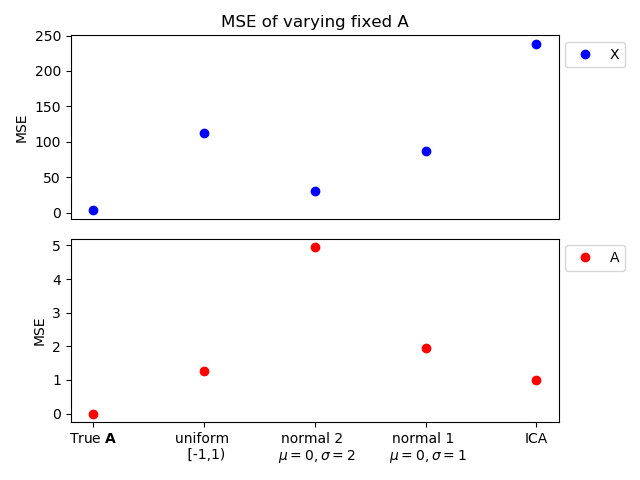
\includegraphics[scale=0.5]{figures/ch_6/A_fix1.png}
\caption{Average MSE values for each of the four fixed mixing matrix $\hat{\mathbf{A}}_{\text{fix}}$ resulting from a stochastic data set specified by $M = 10$, $N = k = 16$ and $L = 1000$.}
\label{fig:vary_A}
\end{figure}
\noindent

\begin{table}[H]
\centering
\begin{tabular}{|c|c|c|c|c|c|}
\hline
 &  $\hat{\mathbf{A}}_{\text{true}}$ & $\hat{\mathbf{A}}_{\text{uni}}$ & $\hat{\mathbf{A}}_{\text{norm2}}$	 & $\hat{\mathbf{A}}_{\text{norm1}}$ & $\hat{\mathbf{A}}_{\text{ICA}}$ \\
\hline
$\text{MSE}(\mathbf{A}, \hat{\mathbf{A}})$ & 0 & 1.271 & 4.957 & 1.941 & 1.006 \\
\hline
$\text{MSE}(\mathbf{X}, \hat{\mathbf{X}})$ & 3.271 & 113.10 & 30.02 & 86.51 & 238.5 \\
\hline
\end{tabular}
\caption{Average MSE values resulting from stochastic data set specified by $M = 10$, $N = k = 16$ and $L = 1000$ with a fixed estimate of the mixing matrix $\hat{\mathbf{A}}_{\text{fix}}$.}
\label{tab:fixed}
\end{table}
\noindent
From table \ref{tab:fixed} and figure \ref{fig:vary_A} it is first of all seen that relation between the MSE of $\mathbf{A}$ and $\mathbf{X}$ is not as expected, as the lowest $\text{MSE}(\mathbf{A}, \hat{\mathbf{A}}_{\text{fix}})$ results in the highest $\text{MSE}(\mathbf{X}, \hat{\mathbf{X}})$ and so forth. 
The lowest $\text{MSE}(\mathbf{A}, \hat{\mathbf{A}}_{\text{fix}})$ is achieved by using $\hat{\mathbf{A}}_{\text{ICA}}$, which confirms that the ICA algorithm manages to estimate $\mathbf{A}$ when $k \leq M$. 
However, as this do not result in the best estimate of $\mathbf{X}$ a different choice of $\hat{\mathbf{A}}$ is still considered. 
The lowest $\text{MSE}(\mathbf{X}, \hat{\mathbf{X}})$ is achieved by use of $\hat{\mathbf{A}}_{\text{norm2}}$, which resulted in the largest $\text{MSE}(\mathbf{A}, \hat{\mathbf{A}}_{\text{fix}})$. 
      
As the main interest in this thesis is to identify the active sources of EEG measurements, a low $\text{MSE}(\mathbf{X}, \hat{\mathbf{X}})$ is more desirable than a low $\text{MSE}(\mathbf{A}, \hat{\mathbf{A}}_{\text{fix}})$. 
Furthermore, a disadvantage of using $\hat{\mathbf{A}}_{\text{ICA}}$ is the limitations in practice when $k = M$ is not possible. 
From these observations a fixed estimate of the mixing matrix drawn from a normal distribution with mean 0 and variance 2, $\hat{\mathbf{A}}_{\text{norm2}}$, is chosen as the alternative estimate of $\mathbf{A}$. 
$\hat{\mathbf{A}}_{\text{norm2}}$ will replace the Cov-DL stage in figure \ref{fig:flow} for following parts the this thesis. 

Due to the unexpected relation between MSE$(\mathbf{A}, \hat{\mathbf{A}}_{\text{fix}})$ and $\text{MSE}(\mathbf{X}, \hat{\mathbf{X}})$ an additional plot is computed. 
Figure \ref{fig:X_func_SNR} shows the average $\text{MSE}(\mathbf{X}, \hat{\mathbf{X}})$ as a function of $\hat{\mathbf{A}}$ with varying SNR value. 
That is an average MSE of 100 realization of the source matrix computed with the true mixing matrix with increasing noise added, the 100 SNR values. 
Additionally figure \ref{fig:A_func_SNR} shows the corresponding average MSE of the 100 realizations between the true $\mathbf{A}$ and estimated $\hat{\mathbf{A}}$ with increasing noise added.
Note that the SNR is decreasing along the x-axis. 

The noise is generated as Gaussian white noise, with increasing variance corresponding to the desired SNR value. 
The SNR value is considered in the interval $[0.01, 2]$. 
From figure \ref{fig:X_func_SNR} it is seen that MSE decreases as the SNR decreases. 
This indicates as first expected that the better estimate of the true mixing matrix $\mathbf{A}$ the better estimate of source matrix $\mathbf{X}$. 
However, this is still a contradiction to the result seen in figure \ref{fig:vary_A}. 
This can however be due to the fact that the true mixing matrix $\mathbf{A}$ being a Gaussian matrix with $\mu = 0$ and $\sigma = 1$ for which Gaussian noise is added. 
The average MSE between the true $\mathbf{A}$ and the noisy $\hat{\mathbf{A}}$ seen in figure \ref{fig:A_func_SNR} is not as high as expected due to the relative large amount of noise. 
All being remarkably less than the corresponding MSE in table \ref{tab:fixed} \todo{Er det ikke varying SNR af true A i figurene?}.  
\begin{figure}[H]
    \begin{minipage}[t]{.45\textwidth}
    	\centering
		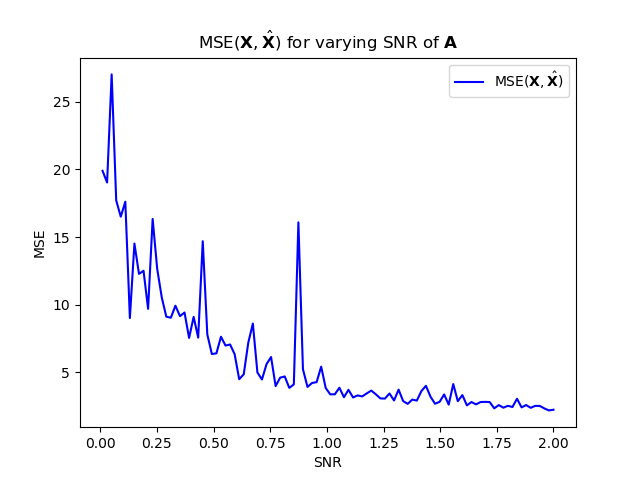
\includegraphics[scale=0.5]{figures/ch_6/X_func_SNR.png}
		\caption{MSE$(\mathbf{X},\hat{\mathbf{X}})$ estimated from stochastic data set specified by $M = 6$, $N = k = 8$ and $L = 1000$, as a function of SNR of given $\mathbf{A}$.}
		\label{fig:X_func_SNR}
    \end{minipage} 
    \hfill
    \begin{minipage}[t]{.45\textwidth}
        \centering
		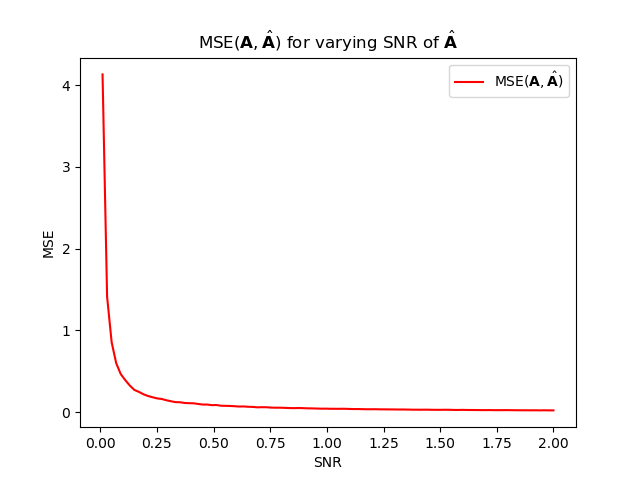
\includegraphics[scale=0.5]{figures/ch_6/A_func_SNR.png}
		\caption{MSE$(\mathbf{A}, \hat{\mathbf{A}})$ where $\hat{\mathbf{A}}$ is a function of the SNR. $\hat{\mathbf{A}}$ correspond to $\hat{\mathbf{A}}$ used in figure \ref{fig:X_func_SNR}.}
		\label{fig:A_func_SNR}
    \end{minipage}
\end{figure}
\noindent